\begin{enumerate}[label=\thechapter.\arabic*,ref=\thechapter.\theenumi]
\item The outputs of four systems $\brak{S_{1} , S_{2} , S_{3},S_{4}}$ corresponding to the input signal $\sin\brak{t}$, for all time $t$ , are shown in the figure. Based on the given information, which of the four systems is/are definately NOT LTI(linear and time-invariant)? 
\begin{figure}[H]
    \resizebox{0.34\textwidth}{!}{\tikzset{
    block/.style = {draw, fill=white, rectangle, minimum height=3em, minimum width=3em}
}

\begin{tikzpicture}[auto, node distance=2cm,>=Latex]

    \node (input) {$\sin\brak{t}$};
    

    \node [block, right=of input] (s1) {$S_{1}$};
    
    \draw[dashed, draw=black] ($(s1.south west) + (-0.2,-0.2)$) rectangle ($(s1.north east) + (0.2,0.2)$);
    \draw [->] (input) -- (s1);
    \draw [->] (s1) -- ++(2,0) node[right]{$\sin\brak{-t}=-\sin\brak{t}$};
    \begin{scope}[yshift=-3cm]
        \node (input2) {$\sin\brak{t}$};
        \node [block, right=of input2] (s2) {$S_{2}$};
        \draw[dashed, draw=black] ($(s2.south west) + (-0.2,-0.2)$) rectangle ($(s2.north east) + (0.2,0.2)$);
        \draw [->] (input2) -- (s2);
        \draw [->] (s2) -- ++(2,0) node[right]{$\sin\brak{t+1}$};
    \end{scope}
    
    \begin{scope}[yshift=-6cm]
        \node (input3) {$\sin\brak{t}$};
        
   
        \node [block, right=of input3] (s3) {$S_{3}$};
        
   
        \draw[dashed, draw=black] ($(s3.south west) + (-0.2,-0.2)$) rectangle ($(s3.north east) + (0.2,0.2)$);
        

        \draw [->] (input3) -- (s3);
        \draw [->] (s3) -- ++(2,0) node[right]{$\sin\brak{2t}$};
    \end{scope}
       \begin{scope}[yshift=-9cm]
        \node (input3) {$\sin\brak{t}$};
        

        \node [block, right=of input3] (s3) {$S_{4}$};
        

        \draw[dashed, draw=black] ($(s3.south west) + (-0.2,-0.2)$) rectangle ($(s3.north east) + (0.2,0.2)$);
        

        \draw [->] (input3) -- (s3);
        \draw [->] (s3) -- ++(2,0) node[right]{$\sin^2\brak{t}$};
    \end{scope}
\end{tikzpicture}

}
    \caption{Block Diagram of Systems}
    \label{fig:question_fig_EC_Q46}
\end{figure}
\hfill(GATE22 EC Q46)\\
\solution
\iffalse
\let\negmedspace\undefined
\let\negthickspace\undefined
\documentclass[journal,12pt,twocolumn]{IEEEtran}
\usepackage{cite}
\usepackage{amsmath,amssymb,amsfonts,amsthm}
\usepackage{algorithmic}
\usepackage{graphicx}
\usepackage{textcomp}
\usepackage{xcolor}
\usepackage{txfonts}
\usepackage{listings}
\usepackage{enumitem}
\usepackage{mathtools}
\usepackage{float}
\usepackage{gensymb}
\usepackage{comment}
\usepackage[breaklinks=true]{hyperref}
\usepackage{tkz-euclide} 
\usepackage{listings}
\usepackage{gvv}                                        
\def\inputGnumericTable{}                                 
\usepackage[latin1]{inputenc}                                
\usepackage{color}                                            
\usepackage{array}          
\usetikzlibrary{positioning, arrows.meta,shapes}
\usepackage{longtable}                                       
\usepackage{calc}                                             
\usepackage{multirow}                                         
\usepackage{hhline}                                           
\usepackage{ifthen}                                           
\usepackage{lscape}
\usepackage{amsmath}
\newtheorem{theorem}{Theorem}[section]
\newtheorem{problem}{Problem}
\newtheorem{proposition}{Proposition}[section]
\newtheorem{lemma}{Lemma}[section]
\newtheorem{corollary}[theorem]{Corollary}
\newtheorem{example}{Example}[section]
\newtheorem{definition}[problem]{Definition}
\newcommand{\BEQA}{\begin{eqnarray}}
\newcommand{\EEQA}{\end{eqnarray}}
\newcommand{\define}{\stackrel{\triangle}{=}}
\theoremstyle{remark}
\newtheorem{rem}{Remark}
\begin{document}

\bibliographystyle{IEEEtran}
\title{GATE-EC-Q46}
\author{EE23BTECH11015 - DHANUSH V NAYAK$^{*}$% <-this % stops a space
}
\maketitle
\newpage
\bigskip
\renewcommand{\thefigure}{\arabic{figure}}
\renewcommand{\thetable}{\theenumi}
\textbf{Question:} The outputs of four systems $\brak{S_{1} , S_{2} , S_{3},S_{4}}$ corresponding to the input signal $\sin\brak{t}$, for all time $t$ , are shown in the figure. Based on the given information, which of the four systems is/are definately NOT LTI(linear and time-invariant)? 
\begin{figure}[H]
    \resizebox{0.34\textwidth}{!}{\tikzset{
    block/.style = {draw, fill=white, rectangle, minimum height=3em, minimum width=3em}
}

\begin{tikzpicture}[auto, node distance=2cm,>=Latex]

    \node (input) {$\sin\brak{t}$};
    

    \node [block, right=of input] (s1) {$S_{1}$};
    
    \draw[dashed, draw=black] ($(s1.south west) + (-0.2,-0.2)$) rectangle ($(s1.north east) + (0.2,0.2)$);
    \draw [->] (input) -- (s1);
    \draw [->] (s1) -- ++(2,0) node[right]{$\sin\brak{-t}=-\sin\brak{t}$};
    \begin{scope}[yshift=-3cm]
        \node (input2) {$\sin\brak{t}$};
        \node [block, right=of input2] (s2) {$S_{2}$};
        \draw[dashed, draw=black] ($(s2.south west) + (-0.2,-0.2)$) rectangle ($(s2.north east) + (0.2,0.2)$);
        \draw [->] (input2) -- (s2);
        \draw [->] (s2) -- ++(2,0) node[right]{$\sin\brak{t+1}$};
    \end{scope}
    
    \begin{scope}[yshift=-6cm]
        \node (input3) {$\sin\brak{t}$};
        
   
        \node [block, right=of input3] (s3) {$S_{3}$};
        
   
        \draw[dashed, draw=black] ($(s3.south west) + (-0.2,-0.2)$) rectangle ($(s3.north east) + (0.2,0.2)$);
        

        \draw [->] (input3) -- (s3);
        \draw [->] (s3) -- ++(2,0) node[right]{$\sin\brak{2t}$};
    \end{scope}
       \begin{scope}[yshift=-9cm]
        \node (input3) {$\sin\brak{t}$};
        

        \node [block, right=of input3] (s3) {$S_{4}$};
        

        \draw[dashed, draw=black] ($(s3.south west) + (-0.2,-0.2)$) rectangle ($(s3.north east) + (0.2,0.2)$);
        

        \draw [->] (input3) -- (s3);
        \draw [->] (s3) -- ++(2,0) node[right]{$\sin^2\brak{t}$};
    \end{scope}
\end{tikzpicture}

}
    \caption{Block Diagram of Systems}
    \label{fig:question_fig_EC_Q46}
\end{figure}
\hfill(GATE22 EC Q46)\\
\solution 
\fi
\begin{table}[H]
\centering
\renewcommand\thetable{1}
\setlength{\extrarowheight}{9pt}
\resizebox{0.4\textwidth}{!}{
\begin{tabular}{|c|c|c|}
\hline
\textbf{Parameter} & \textbf{Description} \\ \hline
$\brak{S_{1} , S_{2} , S_{3},S_{4}}$ & Systems Given  \\ \hline
$\sin\brak{t}$ & Input \\ \hline
$H\brak{\omega}$ & Transfer Function \\ \hline
$X\brak{\omega}$ & Fourier-Transform of input \\ \hline
$Y\brak{\omega}$ & Fourier-Transform of output \\ \hline
$\Phi(\omega)$ & Phase of Transfer Function \\ \hline
\end{tabular}}
\caption{Parameter Table}
\label{tab:gate_ec_Q46}
\end{table}

\begin{figure}[H]
    \resizebox{0.55\textwidth}{!}{\tikzset{
    block/.style = {draw, fill=white, rectangle, minimum height=3em, minimum width=3em}
}

\begin{tikzpicture}[auto, node distance=2cm,>=Latex]
    \node (input) {$x\brak{t}$};
    \node [block, right=of input] (s1) {$H\brak{\omega}$};
    \draw[dashed, draw=black] ($(s1.south west) + (-0.2,-0.2)$) rectangle ($(s1.north east) + (0.2,0.2)$);
    \draw [->] (input) -- (s1);
    \draw [->] (s1) -- ++(2,0) node[right]{$y\brak{t}$};
    \end{tikzpicture}

    }
    \caption{Block Diagram of LTI System}
    \label{fig:LTI_system_EC_q46}
\end{figure}
For an LTI system :
\begin{align}
    y(t)&=h(t)*x(t)\\
    Y\brak{\omega}&=H\brak{\omega}X\brak{\omega}
\end{align}
$H\brak{\omega}$ is a complex exponential :
\begin{align}
    H(j\omega)=\abs{H(j\omega)}e^{j\Phi\brak{\omega}}
\end{align}
$x(t)=\sin\brak{t}$, and $w_{o}=1 rad/sec$
\begin{align}
    X\brak{\omega}&=j\pi \brak{\delta(\omega+\omega_0)-\delta(\omega-\omega_0)}
\end{align}
Now,

\begin{align}
    Y\brak{\omega}=&\brak{\delta(\omega+\omega_0)-\delta(\omega-\omega_0)}\pi \abs{H\brak{\omega}}e^{j\Phi\brak{\omega}}\label{eq:gate22_ec_q46.1}
\end{align}

\begin{align}
    x\brak{t}\delta\brak{t-t_{o}} = x\brak{t_{0}}\delta\brak{t-t_{o}} \label{eq:gate_22_ec_delta_prop_1}
\end{align}
Using property \eqref{eq:gate_22_ec_delta_prop_1} in \eqref{eq:gate22_ec_q46.1} :
\begin{align}
    Y\brak{\omega}=&j\pi \abs{H(-\omega_0)}e^{j\Phi(-\omega_0)}\delta(\omega+\omega_0)\label{eq:gate_ec_q46.3} \\&- j\pi \abs{H\brak{\omega_0}}e^{j\Phi(j\omega_0)}\delta(\omega-\omega_0) \notag 
\end{align}
By definition of the Fourier transform,
\begin{align}
    X(\omega) &= \int_{-\infty}^{\infty} x\brak{t}e^{-j\omega t} \,dt \\
    X^*(\omega) &= \int_{-\infty}^{\infty} x^*(t)e^{j\omega t} \,dt \\
    X^*(-\omega) &= \int_{-\infty}^{\infty} x^*(t)e^{-j\omega t} \,dt\label{eq:gate_ec_q46.2}
\end{align}
For real-time domain signal :
\begin{align}
    x\brak{t} &= x^*\brak{t}
\end{align}
Therefore , from \eqref{eq:gate_ec_q46.2}:
\begin{align}
    X(\omega) =  X^*(-\omega) \label{eq:gate_ec_q46_conjsymm}
\end{align}
By \eqref{eq:gate_ec_q46_conjsymm} , Given $h(t)$ a real-time domain signal, $H\brak{\omega}$ is conjugate symmetric.
\begin{align}
    \abs{H\brak{\omega}}=\abs{H(-\omega)}\label{eq:gate_22_q46_conj_result1}\\
    \Phi(-\omega)=-\Phi\brak{\omega}\label{eq:gate_22_q46_conj_result2}
\end{align}
Therefore using \eqref{eq:gate_22_q46_conj_result1} and \eqref{eq:gate_22_q46_conj_result2} in \eqref{eq:gate_ec_q46.3},
 \begin{align}
    Y\brak{\omega}= j\pi \abs{H\brak{\omega_0}}\brak{e^{-j\Phi\brak{\omega_0}}\delta(\omega+\omega_0) - e^{j\Phi\brak{\omega_0}}\delta(\omega-\omega_0)}
\end{align}
Taking Inverse Fourier Transform, 
\begin{align}
    &\delta(\omega-\omega_0) \system{F} \frac{1}{2}e^{j\omega_0t}\\
     &\delta(\omega+\omega_0) \system{F} \frac{1}{2}e^{-j\omega_0t}\\
    &\implies y(t)=j\pi \abs{H\brak{\omega_0}}\frac{1}{2}\brak{e^{-j\brak{\omega_0t+\Phi\brak{\omega_0}}}-e^{j\brak{\omega_0t+\Phi\brak{\omega_0}}}}\\
    &\implies y(t) =\abs{H\brak{\omega_0}}\sin{\brak{\omega_0t+\Phi\brak{\omega_0}}} 
\end{align}
$w_{0} = 1$ rad/sec :
\begin{align}
    y(t) =\abs{H\brak{1}}\sin{\brak{t+\Phi\brak{1}}} \label{eq:gate_ec_q46_finaloutput}
\end{align}
From \eqref{eq:gate_ec_q46_finaloutput} we can see output cant have scaled frequency nor a squared output. But can have a shifted output or amplitude-scaled output. \\

So, $S_{3}$ and $S_{4}$ cannot be LTI system.
%\end{document}


\pagebreak

    \item The Fourier transform X\brak{j\omega} of the signal\\ $x(t)=\frac{t}{\brak{1+t^2}^2}$ is \rule{1.5cm}{0.15mm}.\hfill{GATE-2022-EC-15}
\begin{enumerate}
	\item[(A)] $\frac{\pi}{2j}\omega e^{-\abs{\omega}}$
	\item[(B)] $\frac{\pi}{2}\omega e^{-\abs{\omega}}$
	\item[(C)] $\frac{\pi}{2j}e^{-\abs{\omega}}$
	\item[(D)] $\frac{\pi}{2}e^{-\abs{\omega}}$
\end{enumerate}

\solution
\iffalse
\let\negmedspace\undefined
\let\negthickspace\undefined
\documentclass[journal,12pt,twocolumn]{IEEEtran}
\usepackage{cite}
\usepackage{amsmath,amssymb,amsfonts,amsthm}
\usepackage{algorithmic}
\usepackage{graphicx}
\usepackage{textcomp}
\usepackage{xcolor}
\usepackage{txfonts}
\usepackage{listings}
\usepackage{enumitem}
\usepackage{mathtools}
\usepackage{gensymb}
\usepackage{comment}
\usepackage[breaklinks=true]{hyperref}
\usepackage{tkz-euclide} 
\usepackage{listings}
\usepackage{gvv}                                        
\def\inputGnumericTable{}                                 
\usepackage[latin1]{inputenc}                                
\usepackage{color}                                            
\usepackage{array}                                            
\usepackage{longtable}                                       
\usepackage{calc}                                             
\usepackage{multirow}                                         
\usepackage{hhline}                                           
\usepackage{ifthen}                                           
\usepackage{lscape}
\usepackage[center]{caption} % center the captions to figure

\newtheorem{theorem}{Theorem}[section]
\newtheorem{problem}{Problem}
\newtheorem{proposition}{Proposition}[section]
\newtheorem{lemma}{Lemma}[section]
\newtheorem{corollary}[theorem]{Corollary}
\newtheorem{example}{Example}[section]
\newtheorem{definition}[problem]{Definition}
\newcommand{\BEQA}{\begin{eqnarray}}
\newcommand{\EEQA}{\end{eqnarray}}
\newcommand{\define}{\stackrel{\triangle}{=}}
\theoremstyle{remark}
\newtheorem{rem}{Remark}
\begin{document}

\newcolumntype{M}[1]{>{\centering\arraybackslash}m{#1}}
\newcolumntype{N}{@{}m{0pt}@{}}

\bibliographystyle{IEEEtran}
\vspace{3cm}

\title{GATE 2022 BM 14 Q} 
\author{ee23btech11223 - Soham Prabhakar More% <-this % stops a space
}
\maketitle
\newpage
\bigskip

\renewcommand{\thefigure}{\theenumi}
\renewcommand{\thetable}{\theenumi}

\bibliographystyle{IEEEtran}

\textbf{Question:} $x\brak{t}$ is a real continuous-time signal whose magnitude frequency response
$\abs{X\brak{j\Omega}}$ is shown below. After sampling $x\brak{t}$ at 100 $rad.s^{-1}$, the spectral point P
is down-converted to \rule{1cm}{0.15mm} $rad.s^{-1}$ in the spectrum of the sampled signal.
\hfill{(GATE 2022 BM 14 Q)}
\begin{figure}[h!]
    \renewcommand\thefigure{1}
    \centering
    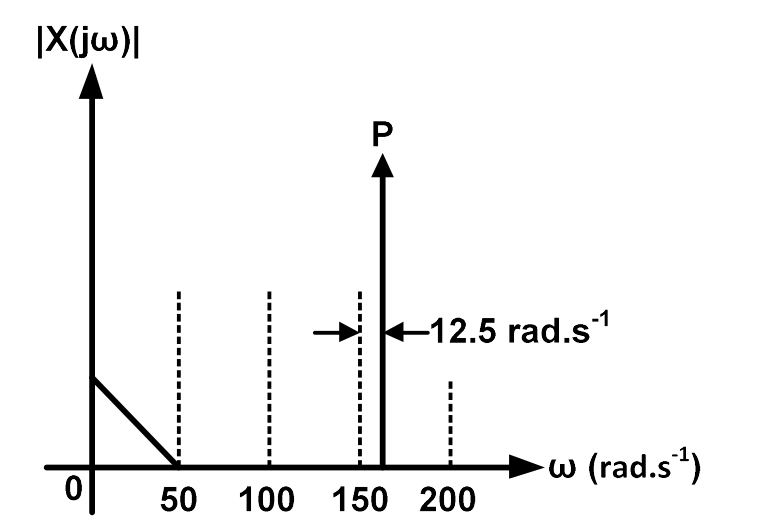
\includegraphics[width=\columnwidth]{2022/BM/14/figs/question.png}
    \caption[short]{Plot of $\abs{X\brak{j\omega}}$}
    \label{fig:2023.bm.14.img1}
\end{figure}

\solution
\fi
\begin{table}[ht]
    \renewcommand\thetable{1}
\begin{tabular}{|c|c|}
    \hline 
    \textbf{Parameter}&\textbf{Description} \\
    \hline
    $w\brak{t}$ & Sampling Function \\
    \hline
	$W\brak{j\omega}$ & Fourier Transform of $w\brak{t}$ \\
    \hline
    $x\brak{t}$ & Input Signal \\
    \hline
    $X\brak{j\omega}$ & Input Signal Frequency Spectrum \\
    \hline
    $x_s\brak{t}$ & Sampled Input Signal \\
    \hline
    $X_s\brak{j\omega}$ & Sampled Signal Frequency Spectrum \\
    \hline
\end{tabular}

\caption{Table of parameters}
\label{Table:1}


\end{table} \\
The sampling function is:
\begin{align}
    w(t) &= \sum_{k = -\infty}^{\infty}\delta\brak{t - \frac{2\pi k}{100}} \\
    W(j\omega) &= 100\sum_{k = -\infty}^{\infty}\delta\brak{j\brak{\omega - 100k}}
\end{align}
then the sampled function: 
\begin{align}
    x_s\brak{t} &= x\brak{t}w\brak{t} \\
    X_s\brak{j\omega} &= X\brak{j\omega} * W\brak{j\omega} \\
    X_s\brak{j\omega} &= \int_{-\infty}^{\infty}X\brak{j\theta}W\brak{j\brak{\omega - \theta}}d\theta \\
    X_s\brak{j\omega} &= 100\sum_{k = -\infty}^{\infty}\int_{-\infty}^{\infty}X\brak{j\theta}\delta\brak{j\brak{\omega - 100k - \theta}}d\theta \\
    X_s\brak{j\omega} &= 100\sum_{k = -\infty}^{\infty}X\brak{j\brak{\omega - 100k}} 
\end{align}
Thus, The down sampled point is at:
\begin{align}
    \omega &= \abs{162.5 - 100k}
\end{align}
where $k$ is the nearest integer to $\frac{162.5}{100}$, which is 2\\
Thus,
\begin{align}
    \omega = 37.5\,rad\,s^{-1}
\end{align}

\begin{figure}[h!]
    \renewcommand\thefigure{2}
    \centering
    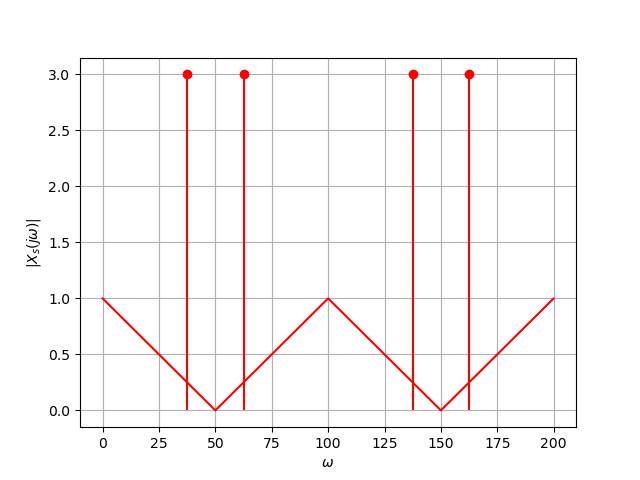
\includegraphics[width=\columnwidth]{2022/BM/14/figs/X_s.png}
    \caption[short]{Plot of $\abs{X_s\brak{j\omega}}$}
    \label{fig:2023.bm.14.img2}
\end{figure}

%\end{document}

\pagebreak

\item For a vector $\bar{x} = [x[0], x[1], \dots, x[7] ]$, the $8$-point discrete Fourier transform (DFT) is denoted by $\bar{X} = \text{DFT}(\bar{x}) = [X[0],X[1],\dots,X[7]]$, where
    \begin{align*}
    X[k] = \sum_{n=0}^{7}x[n]\exp\left(-j\frac{2\pi}{8}nk\right).
    \end{align*} 
    Here $j = \sqrt{-1}$. If $\bar{x} = [1,0,0,0,2,0,0,0]$ and $\bar{y} = \text{DFT}(\text{DFT}(\bar{x}))$, then the value of $y[0]$ is.\hfill{GATE-2022-EC-55}\\
    \solution
    \input{2022/EC/55/55.tex}
    \pagebreak
\item \textbf{Question:} An LTI system is shown in the figure where $$H\brak{s}= \frac{100}{s^2+0.1s+10}$$ The steady state output of the system for an input $x\brak{t}$ is given by $y\brak{t}=a+b\sin{\brak{10t+\theta}}$. The values of $'a'$ and $'b'$ are \\\\
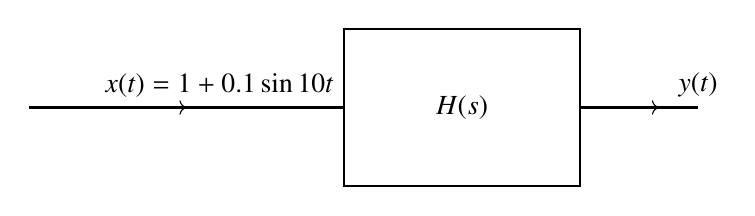
\begin{tikzpicture}
    \draw [thick, draw=black] (-2,-1) -- (2,-1) node[anchor=south east] {$x(t)=1+0.1\sin{\brak{10t}}$};
    \draw [thick,draw=black] (2,0) rectangle (5,-2) ;
    \draw [thick,draw=black] (5,-1) -- (6.5,-1) node[anchor=south] {$y(t)$};
    \draw [->] (-2,-1)--(0,-1);
    \draw [->] (5,-1)--(6,-1);
    \draw (3.5, -1) node[] {$H(s)$};
\end{tikzpicture}\\
\solution 
    \iffalse
\let\negmedspace\undefined
\let\negthickspace\undefined
\documentclass[journal,12pt,twocolumn]{IEEEtran}
\usepackage{cite}
\usepackage{amsmath,amssymb,amsfonts,amsthm}
\usepackage{algorithmic}
\usepackage{graphicx}
\usepackage{textcomp}
\usepackage{xcolor}
\usepackage{txfonts}
\usepackage{listings}
\usepackage{enumitem}
\usepackage{mathtools}
\usepackage{gensymb}
\usepackage{comment}
\usepackage[breaklinks=true]{hyperref}
\usepackage{tkz-euclide} 
\usepackage{listings}
\usepackage{gvv}                                        
\def\inputGnumericTable{}                                 
\usepackage[latin1]{inputenc}                                
\usepackage{color}                                            
\usepackage{array}                                            
\usepackage{longtable}                                       
\usepackage{calc}                                             
\usepackage{multirow}                                         
\usepackage{hhline}                                           
\usepackage{ifthen}                                           
\usepackage{lscape}
\usepackage[center]{caption} % center the captions to figure

\newtheorem{theorem}{Theorem}[section]
\newtheorem{problem}{Problem}
\newtheorem{proposition}{Proposition}[section]
\newtheorem{lemma}{Lemma}[section]
\newtheorem{corollary}[theorem]{Corollary}
\newtheorem{example}{Example}[section]
\newtheorem{definition}[problem]{Definition}
\newcommand{\BEQA}{\begin{eqnarray}}
\newcommand{\EEQA}{\end{eqnarray}}
\newcommand{\define}{\stackrel{\triangle}{=}}
\theoremstyle{remark}
\newtheorem{rem}{Remark}
\begin{document}

\newcolumntype{M}[1]{>{\centering\arraybackslash}m{#1}}
\newcolumntype{N}{@{}m{0pt}@{}}

\bibliographystyle{IEEEtran}
\vspace{3cm}

\title{GATE 2022 BM 14 Q} 
\author{ee23btech11223 - Soham Prabhakar More% <-this % stops a space
}
\maketitle
\newpage
\bigskip

\renewcommand{\thefigure}{\theenumi}
\renewcommand{\thetable}{\theenumi}

\bibliographystyle{IEEEtran}

\textbf{Question:} $x\brak{t}$ is a real continuous-time signal whose magnitude frequency response
$\abs{X\brak{j\Omega}}$ is shown below. After sampling $x\brak{t}$ at 100 $rad.s^{-1}$, the spectral point P
is down-converted to \rule{1cm}{0.15mm} $rad.s^{-1}$ in the spectrum of the sampled signal.
\hfill{(GATE 2022 BM 14 Q)}
\begin{figure}[h!]
    \renewcommand\thefigure{1}
    \centering
    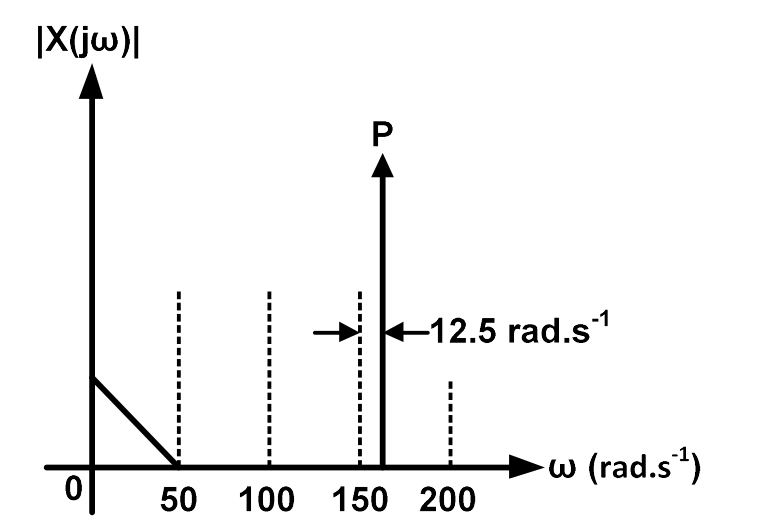
\includegraphics[width=\columnwidth]{2022/BM/14/figs/question.png}
    \caption[short]{Plot of $\abs{X\brak{j\omega}}$}
    \label{fig:2023.bm.14.img1}
\end{figure}

\solution
\fi
\begin{table}[ht]
    \renewcommand\thetable{1}
\begin{tabular}{|c|c|}
    \hline 
    \textbf{Parameter}&\textbf{Description} \\
    \hline
    $w\brak{t}$ & Sampling Function \\
    \hline
	$W\brak{j\omega}$ & Fourier Transform of $w\brak{t}$ \\
    \hline
    $x\brak{t}$ & Input Signal \\
    \hline
    $X\brak{j\omega}$ & Input Signal Frequency Spectrum \\
    \hline
    $x_s\brak{t}$ & Sampled Input Signal \\
    \hline
    $X_s\brak{j\omega}$ & Sampled Signal Frequency Spectrum \\
    \hline
\end{tabular}

\caption{Table of parameters}
\label{Table:1}


\end{table} \\
The sampling function is:
\begin{align}
    w(t) &= \sum_{k = -\infty}^{\infty}\delta\brak{t - \frac{2\pi k}{100}} \\
    W(j\omega) &= 100\sum_{k = -\infty}^{\infty}\delta\brak{j\brak{\omega - 100k}}
\end{align}
then the sampled function: 
\begin{align}
    x_s\brak{t} &= x\brak{t}w\brak{t} \\
    X_s\brak{j\omega} &= X\brak{j\omega} * W\brak{j\omega} \\
    X_s\brak{j\omega} &= \int_{-\infty}^{\infty}X\brak{j\theta}W\brak{j\brak{\omega - \theta}}d\theta \\
    X_s\brak{j\omega} &= 100\sum_{k = -\infty}^{\infty}\int_{-\infty}^{\infty}X\brak{j\theta}\delta\brak{j\brak{\omega - 100k - \theta}}d\theta \\
    X_s\brak{j\omega} &= 100\sum_{k = -\infty}^{\infty}X\brak{j\brak{\omega - 100k}} 
\end{align}
Thus, The down sampled point is at:
\begin{align}
    \omega &= \abs{162.5 - 100k}
\end{align}
where $k$ is the nearest integer to $\frac{162.5}{100}$, which is 2\\
Thus,
\begin{align}
    \omega = 37.5\,rad\,s^{-1}
\end{align}

\begin{figure}[h!]
    \renewcommand\thefigure{2}
    \centering
    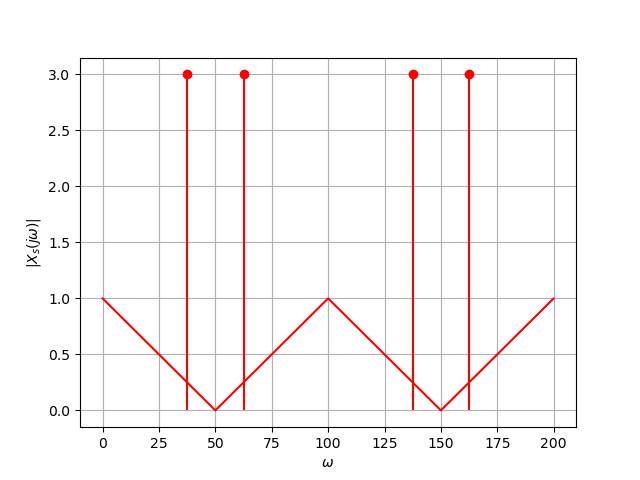
\includegraphics[width=\columnwidth]{2022/BM/14/figs/X_s.png}
    \caption[short]{Plot of $\abs{X_s\brak{j\omega}}$}
    \label{fig:2023.bm.14.img2}
\end{figure}

%\end{document}

\item A periodic function $f(x)$, with period 2, is defined as \\
   \begin{align}   
   f(x) =
   \begin{cases}
    -1-x & -1 \leq x<0 \\
     1-x &  0 <x \leq1 
   \end{cases}
   \end{align} 
   The Fourier series of this function contains \\
\begin{enumerate}[label=\Alph*.]
\item Both $\cos(n\pi x)$ and $sin(n\pi x)$ where n=1,2,3...
\item Only $\sin(n\pi x)$ where n=1,2,3...
\item Only $\cos(n\pi x)$ where n=1,2,3...
\item Only $\cos(2n\pi x)$ where n=1,2,3...  \hfill{GATE IN 2022 }
\end{enumerate} 

\solution
\input{2022/IN/13/g13.tex}
\item  A Simple closed path C in the Complex Plane is shown in the figure.
 \begin{align*}
        \oint_C \frac{2^z}{z^2-1}dz=-\jmath \pi A
 \end{align*}
 Where $\jmath=\sqrt{-1}$, Then find the value of A is \rule{1cm}{0.15mm}(Rounded of to two decimals)
\begin{figure}[h!]
    \centering
    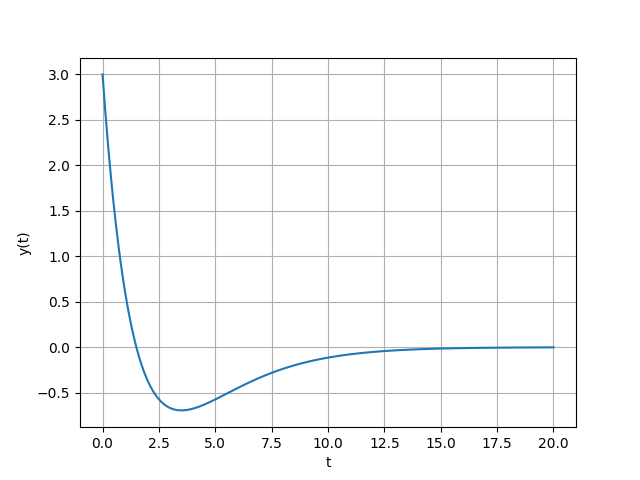
\includegraphics[width = \columnwidth]{2022/EC/32/figs/fig1.png}
\end{figure}
\hfill{(GATE 2022 EC)}\\
\solution 
\input{2022/EC/32/EC_32.tex}
\pagebreak
\item For the ideal AC-DC rectifier circuit shown in the figure below, the load current
magnitude is $I_{dc}$ = $15$ A and is ripple free. The thyristors are fired with a delay angle
of 45\degree
. The amplitude of the fundamental component of the source current, in
amperes, is \_\_\_\_\_\_\_\_{\em (Round off to 2
decimal places)}. \hfill(GATE 59 EE 2022)
\begin{figure}[!h]
\centering
 \begin{circuitikz}[scale = 0.8]
      \draw (-0.8,0.8) -- (-0.8,0.8) node[above]{$+$};
    \draw (0,2) to[sV] (0,-1);
     \draw (-0.8,0) -- (-0.8,0) node[below]{$-$};
    \draw (0,2) -- (2,2);
    \draw (2,2) -- (2,1);
    \draw (2,1) -- (3,1);
     \draw (3,1) to [thyristor] (3,3);
    \draw (3,3) -- (5,3);
    \draw (5,1) to [thyristor] (5,3);
    \draw (5,3) -- (7,3);
    \draw (7,3) to[resistor](7,1);
    \draw (7,1) -- (7,0);
    \draw(7,0) to [L](7,-2);
    \draw (7,-2) -- (3,-2);

    \draw (0, -1) -- (2,-1);
    \draw (2,-1) -- (2,0.4);
    \draw (2,0.4) -- (5,0.4);
    \draw (3,-2) to [Do] (3,0.4);
    \draw (3,0.4) -- (3,1);
    \draw (5,-2) to [Do] (5,0.4);
    \draw (5,0.4) -- (5,1);

     \draw[->] (6.5, 2) -- (6.5, 1) node[midway, left]{$I_{dc}$};
        \end{circuitikz}
\end{figure}
\solution

 \iffalse
\let\negmedspace\undefined
\let\negthickspace\undefined
\documentclass[journal,12pt,onecolumn]{IEEEtran}
\usepackage{cite}
\usepackage{amsmath,amssymb,amsfonts,amsthm}
\usepackage{algorithmic}
\usepackage{graphicx}
\usepackage{textcomp}
\usepackage{xcolor}
\usepackage{txfonts}
\usepackage{listings}
\usepackage{enumitem}
\usepackage{mathtools}
\usepackage{gensymb}
\usepackage{comment}
\usepackage[breaklinks=true]{hyperref}
\usepackage{tkz-euclide} 
\usepackage{tikz}
\usepackage{circuitikz}
%\usetikzlibrary{circuits.ee.IEC}
\usepackage{listings}
\usepackage{gvv} 
\usepackage{caption}
\def\inputGnumericTable{}                   

%\usepackage[latin1]{inputenc}                                
\usepackage{color}                                            
\usepackage{array}                                            
\usepackage{longtable}                                       
\usepackage{calc}                                             
\usepackage{multirow}                                         
\usepackage{hhline}                                           
\usepackage{ifthen}                                           
\usepackage{lscape}
\usepackage{tikz}
\usepackage{circuitikz}

\newtheorem{theorem}{Theorem}[section]
\newtheorem{problem}{Problem}
\newtheorem{proposition}{Proposition}[section]
\newtheorem{lemma}{Lemma}[section]
\newtheorem{corollary}[theorem]{Corollary}
\newtheorem{example}{Example}[section]
\newtheorem{definition}[problem]{Definition}
\newcommand{\BEQA}{\begin{eqnarray}}
\newcommand{\EEQA}{\end{eqnarray}}
\newcommand{\define}{\stackrel{\triangle}{=}}
\theoremstyle{remark}
\newtheorem{rem}{Remark}

\begin{document}

\bibliographystyle{IEEEtran}
\vspace{3cm}

\title{GATE: EE - 59.2022}
\author{EE23BTECH11013 - Avyaaz$^{*}$% <-this % stops a space 
}
\maketitle
% \newpage
% \bigskip

\renewcommand{\thefigure}{\arabic{figure}}
\renewcommand{\thetable}{\arabic{table}}

\large\textbf{\textsl{Question:}}
For the ideal AC-DC rectifier circuit shown in the figure below, the load current
magnitude is $I_{dc}$ = $15$ A and is ripple free. The thyristors are fired with a delay angle
of 45\degree
. The amplitude of the fundamental component of the source current, in
amperes, is \_\_\_\_\_\_\_\_{\em (Round off to 2
decimal places)}. \hfill(GATE 59 EE 2022)
\begin{figure}[!h]
\centering
 \begin{circuitikz}[scale = 0.8]
      \draw (-0.8,0.8) -- (-0.8,0.8) node[above]{$+$};
    \draw (0,2) to[sV] (0,-1);
     \draw (-0.8,0) -- (-0.8,0) node[below]{$-$};
    \draw (0,2) -- (2,2);
    \draw (2,2) -- (2,1);
    \draw (2,1) -- (3,1);
     \draw (3,1) to [thyristor] (3,3);
    \draw (3,3) -- (5,3);
    \draw (5,1) to [thyristor] (5,3);
    \draw (5,3) -- (7,3);
    \draw (7,3) to[resistor](7,1);
    \draw (7,1) -- (7,0);
    \draw(7,0) to [L](7,-2);
    \draw (7,-2) -- (3,-2);

    \draw (0, -1) -- (2,-1);
    \draw (2,-1) -- (2,0.4);
    \draw (2,0.4) -- (5,0.4);
    \draw (3,-2) to [Do] (3,0.4);
    \draw (3,0.4) -- (3,1);
    \draw (5,-2) to [Do] (5,0.4);
    \draw (5,0.4) -- (5,1);

     \draw[->] (6.5, 2) -- (6.5, 1) node[midway, left]{$I_{dc}$};
        \end{circuitikz}

\end{figure}

\solution
\fi
\begin{table}[htbp]
\setlength{\extrarowheight}{4pt}
\setlength{\tabcolsep}{3pt}
\centering
\begin{tabular}{|c|c|c|}
\hline
\textbf{Parameter} & \textbf{Description}&\textbf{Value}\\
\hline 
$I_{dc}$& Load current & $15$A  \\
\hline
$\alpha$ &Firing angle&$45\degree$ \\
\hline
\end{tabular}

\caption{}
\label{tab:inputs.EE.59.2022}
\end{table}
% It is a Single phase symmetrical semi-converter.
% \begin{enumerate}[label={\roman*)}]
%     \item Load current magnitude $\brak{I_{dc}}$ = $15$A
%     \item Firing angle $\brak{\alpha} = 45\degree$
% \end{enumerate}
A symmetrical single phase semi converter is shown below,

\begin{figure}[!h]
\centering
    \begin{circuitikz}[scale = 0.8]
      \draw (-0.8,0.8) -- (-0.8,0.8) node[above]{$+$};
    \draw (0,2) to[sV,l=$V_s$] (0,-1);
     \draw (-0.8,0) -- (-0.8,0) node[below]{$-$};
    \draw (0,2) -- (2,2);
    \draw (2,2) -- (2,1);
    \draw (2,1) -- (3,1);
     \draw (3,1) to [thyristor] (3,3);
     \node at (2.4,2.3) {$T_1$};
    \draw (3,3) -- (5,3);
    \draw (5,1) to [thyristor] (5,3);
     \node at (4.4,2.3) {$T_2$};
    \draw (5,3) -- (7,3);
    \draw (7,3) to[resistor](7,1);
    \draw (7,1) -- (7,0);
    \draw(7,0) to [L](7,-2);
    \draw (7,-2) -- (3,-2);

    \draw (0, -1) -- (2,-1);
    \draw (2,-1) -- (2,0.4);
    \draw (2,0.4) -- (5,0.4);
    \draw (3,-2) to [Do] (3,0.4);
    \node at (3.8,-1) {$D_1$};
    \draw (3,0.4) -- (3,1);
    \draw (5,-2) to [Do] (5,0.4);
    \node at (5.8,-1) {$D_2$};
    \draw (5,0.4) -- (5,1);

     \draw[->] (6.5, 2) -- (6.5, 1) node[midway, left]{$I_{dc}$};
          \draw[->] (0.5, 2) -- (1, 2) ;
          \node at (1,1.6) {$I_s$};
          \node at (7.4,2) {$R$};
          \node at (7.4,-1.1) {$L$};

     \draw (8,2.8) -- (8,2.8) node[above]{$+$};
     \draw[->] (8,0.8) -- (8,2.8);
     \node at (8,0.5) {$V_o$};
     \draw[->] (8,0.2) -- (8,-1.8);
     \draw (8,-1.8) -- (8,-1.8) node[below]{$-$};
        \end{circuitikz}

\end{figure}

The Fourier series representation of supply current is given by:
\begin{align}
    i_s(t) = a_o +\sum_{n=1}^{\infty}C_n\sin({n\omega t} + \theta_n)\label{eq:gen_i_s}
\end{align}
 where,
 \begin{align}
 a_o &= \frac{1}{2\pi} \int_{0}^{2\pi} i_s(t)d\omega t \\
     C_n &= \sqrt{a_n^2 + b_n ^2}\label{eq:bino_coeff}\\
     \theta_n &= \tan^{-1}\left({\frac{a_n}{b_n}}\right)\label{eq: theta}
 \end{align}
\begin{align}
  \implies  a_o &= \frac{1}{2\pi}\int_{\alpha}^{\pi} I_o d\omega t - \int_{\pi + \alpha}^{2\pi} I_o d\omega t = 0\\
 \implies   a_n &= \frac{1}{\pi} \int_{\alpha}^{\pi}I_o\cos n\omega t d\omega t - \int_{\pi + \alpha}^{2\pi} I_o\cos{n\omega td\omega t}\\
 a_n &= 
 \begin{cases}
    \frac{-2I_o}{n\pi}\sin{n\alpha} & \text{for } n = 1,3,5...\\
     0 &\text{for } n = 2,4.....
    \end{cases}\\
 \implies   b_n &= \frac{1}{\pi}\int_{\alpha}^{\pi}I_o\sin n\omega t d\omega t - \int_{\pi + \alpha}^{2\pi} I_o\sin{n\omega td\omega t} \\
 b_n &= 
 \begin{cases}
     \frac{2I_o}{n\pi}\left(1 + \cos{n\alpha}\right) &\text{for } n = 1,3,5...\\
     0 &\text{for } n = 2, 4....
    \end{cases}
    \end{align}
From \eqref{eq:bino_coeff}:
\begin{align}
  \therefore  C_n &= \frac{2\sqrt{2}I_o}{n\pi}\left(\sqrt{1 + \cos{n\alpha}}\right)\\
  \implies  C_n &= \frac{4I_o}{n\pi}\cos{\frac{n\alpha}{2}}\label{eq:final_bino}
\end{align}
From \eqref{eq: theta}:
\begin{align}
    \theta_n &= \tan^{-1}\left(\frac{-\sin{n\alpha}}{1 + \cos{n\alpha}}\right)\\
    \implies \theta_n &= \frac{-n\alpha}{2}\label{eq:final_theta}
\end{align}

From \eqref{eq:gen_i_s},\eqref{eq:final_bino} and \eqref{eq:final_theta}:
\begin{align}
I_{s}(t) = \sum_{n=1,3,5...}^{\infty} \frac{4I_{o}}{n\pi}\cos{\frac{n\alpha}{2}}\sin{\left(n\omega t - \frac{n\alpha}{2}\right)}
\end{align}
% \begin{align}
% I_{s}(t) = \sum_{n=1,3,5...}^{\infty} \frac{4I_{dc}}{n\pi}\cos{\frac{n\alpha}{2}}\sin{\left(n\omega t - \frac{n\alpha}{2}\right)}
% \end{align}


% \begin{tikzpicture}[scale=1]
%     \draw[->] (0,0) -- (10,0) node[right] {$\omega t$};
%     \draw[->] (0,-2) -- (0,2) node[above] {$y$};
%     \draw[domain=0:10, smooth, variable=\x, black] plot ({\x},{sin(deg(\x))});
%     \foreach \x/\xtext in {1.57/\frac{\pi}{2},3.14/\pi,4.71/\frac{3\pi}{2},6.28/2\pi,7.85/\frac{7\pi}{2}} {
%         \draw (\x cm,0) -- (\x cm,0.1) node[below] {$\xtext$};
%     }
%     \foreach \y in {-1,1} {
%         \draw (1pt,\y cm-1.5) -- (-1pt,\y cm-1.5) node[left] {$\y$};
%     }
% \end{tikzpicture}

\begin{figure}[!h]
    \centering
    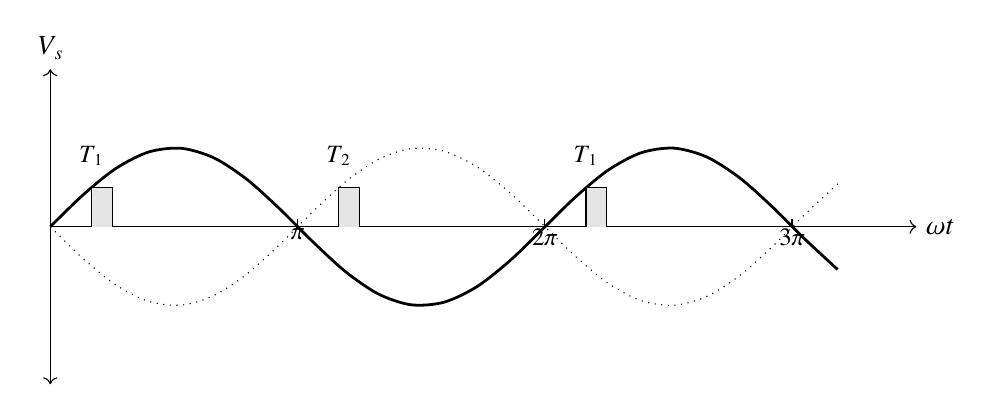
\begin{tikzpicture}[scale=1]
    \draw[->] (0,0) -- (11,0) node[right] {$\omega t$};
    \draw[<->] (0,-2) -- (0,2) node[above] {$V_s$};
    \draw[domain=0:10, smooth, variable=\x, black,line width=1pt] plot ({\x},{sin(deg(\x))});
    \draw[dotted,domain=0:10, smooth, variable=\x, black] plot ({\x},{-sin(deg(\x))});
    \foreach \x/\xtext in {3.14/\pi,6.28/2\pi,9.42/3\pi} {
        \draw (\x cm,0) -- (\x cm,0.1) node[below] {\small$\xtext$};
    }

\fill[gray!20] (0.5233,0) -- (0.5233,0.5) -- (0.785,0.5) -- (0.785,0) -- cycle;
    \fill[gray!20] (3.6633,0) -- (3.6633,0.5) -- (3.925,0.5) -- (3.925,0) -- cycle;
    \fill[gray!20] (6.8033,0) -- (6.8033,0.5) -- (7.065,0.5) -- (7.065,0) -- cycle;

    \draw (0.5233,0) -- (0.5233,0.5);
    \draw (0.5233,0.5) -- (0.785,0.5);
    \draw (0.785,0.5) -- (0.785,0);

    \draw (3.6633,0) -- (3.6633,0.5);
    \draw (3.6633,0.5) -- (3.925,0.5);
    \draw (3.925,0.5) -- (3.925,0);

    \draw (6.8033,0) -- (6.8033,0.5);
    \draw (6.8033,0.5) -- (7.065,0.5);
    \draw (7.065,0.5) -- (7.065,0);


     \node at (0.5233,0.9) {\small$T_1$};
     \node at (3.6633,0.9) {\small$T_2$};
     \node at (6.8033,0.9) {\small$T_1$};
\end{tikzpicture}
\end{figure}
\begin{figure}[!h]
    \centering
    \begin{tikzpicture}[scale=1]
    \draw[->] (0,0) -- (11,0) node[right] {$\omega t$};
    \draw[<->] (0,-2) -- (0,2) node[above] {$V_o$};
    \draw[domain=0.5233:3.14, smooth, variable=\x, black,line width=1pt] plot ({\x},{sin(deg(\x))});
    \draw[domain=3.6633:6.28, smooth, variable=\x, black,line width=1pt] plot ({\x},{-sin(deg(\x))});
    \draw[domain=6.8033:9.42, smooth, variable=\x, black,line width=1pt] plot ({\x},{sin(deg(\x))});

    \foreach \x/\xtext in {0.5233/\alpha, 3.14/\pi,4/\pi + \alpha ,6.28/2\pi,7.2/2\pi + \alpha,9.42/3\pi}{
        \draw (\x cm,0) -- (\x cm,0) node[below] {\small $\xtext$};
    }

     \draw [line width=1pt](0,0)--(0.5233,0);
    \draw [line width=1pt](0.5233,0) -- (0.5233,0.5);
    \draw[line width=1pt](3.14,0)-- (3.6633,0);
    \draw[line width=1pt] (3.6633,0) -- (3.6633,0.5);
    \draw [line width=1pt](6.28,0)--(6.8033,0);
    \draw [line width=1pt](6.8033,0) -- (6.8033,0.5);

    \node at (0.25,0.6){\small$T_2$};
    \node at (0.25,0.2){\small$D_2$};
     \node at (3.4,0.6){\small$T_1$};
    \node at (3.4,0.2){\small$D_1$};
    \node at (6.4,0.6){\small$T_2$};
    \node at (6.4,0.2){\small$D_2$};

    \node at (1.57,0.4){\small $T_1D_2$};
    \node at (4.71,0.4){\small $T_2D_1$};
    
\end{tikzpicture}
\end{figure}
\begin{figure}[!h]
    \centering
    \begin{tikzpicture}[scale=1]
    \draw[->] (0,0) -- (11,0) node[right] {$\omega t$};
    \draw[<->] (0,-2) -- (0,2) node[above] {$i_{T_1}$};
   
    \foreach \x/\xtext in {0.5233/\alpha,4/\pi + \alpha,7.2/2\pi + \alpha,10/3\pi + \alpha}{
        \draw (\x cm,0) -- (\x cm,0) node[below] {\small $\xtext$};
    }
     \draw [line width=1pt](0,0)--(0.5233,0);
    \draw [line width=1pt](0.5233,0) -- (0.5233,1);
    \draw[line width=1pt](0.5233,1)-- (3.6633,1);
    \draw[line width=1pt] (3.6633,1) -- (3.6633,0);
    \draw[line width=1pt] (3.6633,0) -- (6.8033,0);
    \draw [line width=1pt](6.8033,0)--(6.8033,1);
    \draw [line width=1pt](6.8033,1) -- (9.948,1);
     \draw [line width=1pt] (9.948,1) -- (9.948,0);

     \draw[dotted,domain=0:10, smooth, variable=\x, black] plot ({\x},{1});
     \node at (0.4,1.2) {\small $I_{DC}$};
\end{tikzpicture}
\end{figure}
\begin{figure}[!h]
    \centering
    \begin{tikzpicture}[scale=1]
    \draw[->] (0,0) -- (11,0) node[right] {$\omega t$};
    \draw[<->] (0,-2) -- (0,2) node[above] {$i_{s}$};
   

    \draw [line width=1pt](0.5233,0) -- (0.5233,1);
    \draw[line width=1pt](0.5233,1)-- (3.14,1);
    \draw[line width=1pt](3.14,1)-- (3.14,0);
    \draw[line width=1pt] (3.14,0) -- (3.6633,0);
    \draw[line width=1pt] (3.6633,0) -- (3.6633,-1);
    \draw[line width=1pt] (3.6633,-1) -- (6.28,-1);
    \draw[line width=1pt]  (6.28,-1) -- (6.28,0);
    \draw[line width=1pt] (6.28,0) -- (6.8033,0);
    \draw [line width=1pt](6.8033,0)--(6.8033,1);
    \draw [line width=1pt](6.8033,1) -- (9.42,1);
     \draw [line width=1pt] (9.42,1) -- (9.42,0);
     \draw [line width=1pt] (9.42,0) -- (9.948,0);

     \draw[dotted,domain=0:10, smooth, variable=\x, black] plot ({\x},{1});
     \node at (0.4,1.2) {\small $I_{DC}$};
    
\end{tikzpicture}
\end{figure}

From \tabref{tab:inputs.EE.59.2022}:
\begin{align}
   (I_{s_1})_{peak} &= \frac{4I_{dc}}{\pi}\cos{\left(\frac{\alpha}{2}\right)}\\
    &= \frac{4 \times 15 }{\pi}\times \cos{\frac{45 \degree}{2}}\\
    &=17.64 A 
\end{align}


\pagebreak

\item If 
\begin{align}
    \frac{a_0}{2} + \sum_{n=1}^{\infty}a_n\cos(nx)\nonumber
\end{align}
is the Fourier cosine series of the function
\begin{align}
    f(x) = \sin(x), 0 < x < \pi \nonumber
\end{align}
then which of the following are TRUE?
\begin{enumerate}[label=(\alph*)]
    \item $a_0 + a_1 = \frac{4}{\pi}$
    \item $a_0 = \frac{4}{\pi}$
    \item $a_0 + a_1 = \frac{2}{\pi}$
    \item $a_1 = \frac{2}{\pi}$
\end{enumerate}
\hfill(GATE 2022 NM Q24)\\
\solution
\input{2022/NM/24/GATE_NM_22_24.tex}
\pagebreak

\item The fourier series expansion of $x^3$ in the interval $-1\leq x\leq 1$with periodic continuation has
\begin{enumerate}[label=(\alph*)]
    \item only sine terms
    \item only cosine terms
    \item both sine and cosine terms
    \item only sine terms and a non-zero constant
\end{enumerate} \hfill(GATE 2022 ME)    \\
\solution
\input{2022/ME/14/gate6.tex}
\pagebreak

\item The discrete time Fourier series representation of a signal $x[n]$ with period $N$ is written as  $x[n]=\sum_{k=0}^{N-1}a_ke^{j\brak{2kn\pi/N}}$ . A discrete time periodic signal with period $N=3$, has the non-zero Fourier series coefficients: $a_{-3}=2$ and $a_4=1$. The signal is
\begin{enumerate}[label=(\Alph*)]
\item $2+2e^{-\brak{j\frac{2\pi}{6}n}}\cos{\brak{\frac{2\pi}{6}n}}$
\item $1+2e^{\brak{j\frac{2\pi}{6}n}}\cos{\brak{\frac{2\pi}{6}n}}$
\item $1+2e^{\brak{j\frac{2\pi}{3}n}}\cos{\brak{\frac{2\pi}{6}n}}$
\item $2+2e^{\brak{j\frac{2\pi}{6}n}}\cos{\brak{\frac{2\pi}{6}n}}$
\end{enumerate}
\hfill(GATE EE 2022)
\\
\solution
\input{2022/EE/49/49.tex}
\pagebreak

\item Consider the wave elevation spectrum $S_{\eta \eta}(\omega)$ as shown in the figure. Then, the significant wave height is \underline{\hspace{3cm}} m.
\begin{figure}[H]
    \centering
    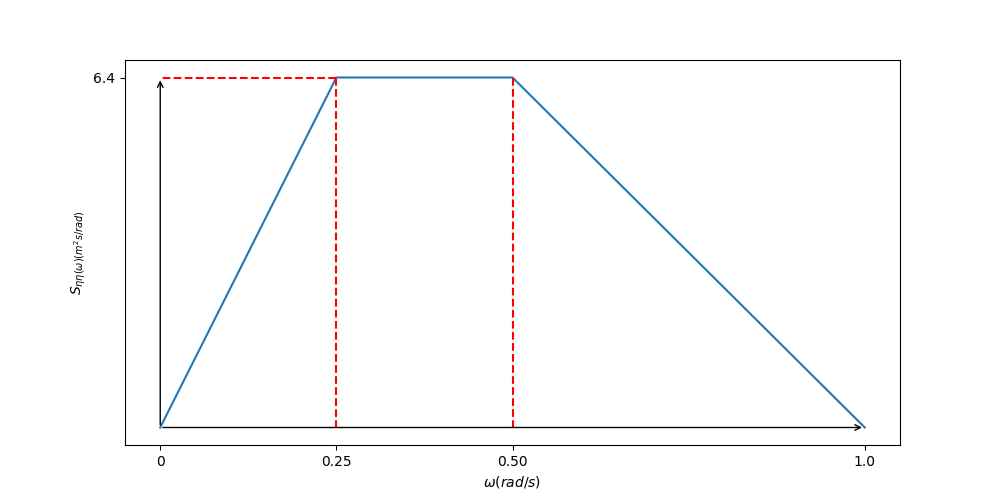
\includegraphics[width=\columnwidth]{2022/NM/40/figs/qfig.png}
    \caption{Wave Elevation Spectrum}
    \label{fig: GATE22NM40.1}
\end{figure}

\begin{enumerate}[label=(\Alph*)]
\item 2
\item 4
\item 6
\item 8
\end{enumerate}
\hfill{GATE NM 2022} \\
\solution \\
\iffalse
\let\negmedspace\undefined
\let\negthickspace\undefined

\documentclass[journal,12pt,onecolumn]{IEEEtran}

\usepackage{cite}
\usepackage{amsmath,amssymb,amsfonts,amsthm}
\usepackage{graphicx}
\usepackage{textcomp}
\usepackage{xcolor}
\usepackage{txfonts}
\usepackage{listings}
\usepackage{enumitem}
\usepackage{mathtools}
\usepackage{gensymb}
\usepackage[breaklinks=true]{hyperref}
\usepackage{tkz-euclide}
\usepackage{listings}
\usepackage{float}

\newtheorem{theorem}{Theorem}[section]
\newtheorem{problem}{Problem}
\newtheorem{proposition}{Proposition}[section]
\newtheorem{lemma}{Lemma}[section]
\newtheorem{corollary}[theorem]{Corollary}
\newtheorem{example}{Example}[section]
\newtheorem{definition}[problem]{Definition}
\newcommand{\BEQA}{\begin{eqnarray}}
\newcommand{\EEQA}{\end{eqnarray}}
\newcommand{\define}{\stackrel{\triangle}{=}}
\theoremstyle{remark}
\newtheorem{rem}{Remark}

\begin{document}

\providecommand{\pr}[1]{\ensuremath{\Pr\left(#1\right)}}
\providecommand{\prt}[2]{\ensuremath{p_{#1}^{\left(#2\right)} }}
\providecommand{\qfunc}[1]{\ensuremath{Q\left(#1\right)}}
\providecommand{\sbrak}[1]{\ensuremath{{}\left[#1\right]}}
\providecommand{\lsbrak}[1]{\ensuremath{{}\left[#1\right.}}
\providecommand{\rsbrak}[1]{\ensuremath{{}\left.#1\right]}}
\providecommand{\brak}[1]{\ensuremath{\left(#1\right)}}
\providecommand{\lbrak}[1]{\ensuremath{\left(#1\right.}}
\providecommand{\rbrak}[1]{\ensuremath{\left.#1\right)}}
\providecommand{\cbrak}[1]{\ensuremath{\left\{#1\right\}}}
\providecommand{\lcbrak}[1]{\ensuremath{\left\{#1\right.}}
\providecommand{\rcbrak}[1]{\ensuremath{\left.#1\right\}}}
\newcommand{\sgn}{\mathop{\mathrm{sgn}}}
\providecommand{\abs}[1]{\left\vert#1\right\vert}
\providecommand{\res}[1]{\Res\displaylimits_{#1}} 
\providecommand{\norm}[1]{\left\lVert#1\right\rVert}
\providecommand{\mtx}[1]{\mathbf{#1}}
\providecommand{\mean}[1]{E\left[ #1 \right]}
\providecommand{\cond}[2]{#1\middle|#2}
\providecommand{\fourier}{\overset{\mathcal{F}}{ \rightleftharpoons}}
\newenvironment{amatrix}[1]{%
  \left(\begin{array}{@{}*{#1}{c}|c@{}}
}{%
  \end{array}\right)
}
\newcommand{\solution}{\noindent \textbf{Solution: }}
\newcommand{\cosec}{\,\text{cosec}\,}
\providecommand{\dec}[2]{\ensuremath{\overset{#1}{\underset{#2}{\gtrless}}}}
\newcommand{\myvec}[1]{\ensuremath{\begin{pmatrix}#1\end{pmatrix}}}
\newcommand{\mydet}[1]{\ensuremath{\begin{vmatrix}#1\end{vmatrix}}}
\newcommand{\myaugvec}[2]{\ensuremath{\begin{amatrix}{#1}#2\end{amatrix}}}
\providecommand{\rank}{\text{rank}}
\providecommand{\pr}[1]{\ensuremath{\Pr\left(#1\right)}}
\providecommand{\qfunc}[1]{\ensuremath{Q\left(#1\right)}}
	\newcommand*{\permcomb}[4][0mu]{{{}^{#3}\mkern#1#2_{#4}}}
\newcommand*{\perm}[1][-3mu]{\permcomb[#1]{P}}
\newcommand*{\comb}[1][-1mu]{\permcomb[#1]{C}}
\providecommand{\qfunc}[1]{\ensuremath{Q\left(#1\right)}}
\providecommand{\gauss}[2]{\mathcal{N}\ensuremath{\left(#1,#2\right)}}
\providecommand{\diff}[2]{\ensuremath{\frac{d{#1}}{d{#2}}}}
\providecommand{\myceil}[1]{\left \lceil #1 \right \rceil }
\newcommand\figref{Fig.~\ref}
\newcommand\tabref{Table~\ref}
\newcommand{\sinc}{\,\text{sinc}\,}
\newcommand{\rect}{\,\text{rect}\,}
\let\vec\mathbf
\bibliographystyle{IEEEtran}
\bigskip
Q: Consider the wave elevation spectrum $S_{\eta \eta}(\omega)$ as shown in the figure. Then, the significant wave height is \underline{\hspace{3cm}} m.
\begin{figure}[H]
    \centering
    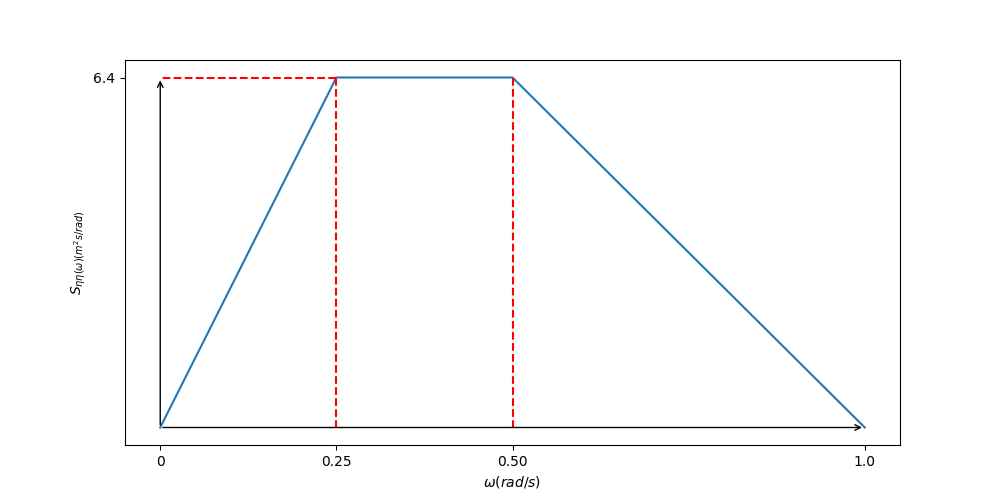
\includegraphics[width=\columnwidth]{2022/NM/40/figs/qfig.png}
    \caption{Wave Elevation Spectrum}
    \label{fig: GATE22NM40.1}
\end{figure}

\begin{enumerate}[label=(\Alph*)]
\item 2
\item 4
\item 6
\item 8
\end{enumerate}
\hfill{GATE NM 2022}


\solution
\fi
Given:
\begin{align}
S_{\eta \eta}(\omega)(m^2s/rad) = 
\begin{cases}
  25.6\omega   & \text{if } \omega \in [0,0.25] \\
  6.4  & \text{if } \omega \in (0.25,0.50] \\
  12.8\omega-12.8  & \text{if } \omega \in (0.50,1.0] \\
  0  & o.w \\
\end{cases}
\end{align}
In terms of f:
\begin{align}
S_{\eta \eta}(f)(m^2s) = 
\begin{cases}
  51.2\pi f   & \text{if } f \in [0,\frac{\pi}{2}] \\
  6.4  & \text{if } f \in (\frac{\pi}{2},\pi] \\
  25.6\pi f-12.8  & \text{if } f \in (\pi,2\pi] \\
  0 & o.w \\
\end{cases} \label{eq: GATE22NM40.1}
\end{align}
Significant Wave Height:
\begin{align}
H_s &= 4 \sqrt{\int_{0}^{\infty} S(f)df}
\end{align}
From \eqref{eq: GATE22NM40.1}
\begin{align}
H_s &= 4 \sqrt{\int_{0}^{\frac{\pi}{2}} 51.2\pi fdf + \int_{\frac{\pi}{2}}^{\pi} 6.4df + \int_{\pi}^{2\pi} (25.6\pi f-12.8)df} \\
&= 4 \sqrt{0.8 +1.6 +1.6} \\
\therefore H_s &= 8
\end{align}
Hence the answer is option (D).
%table
%\begin{table}[!h]
%\begin{tabular}[12pt]{ |c| c|c|}
    \hline
    \textbf{Parameter} & \textbf{Description} & \textbf{Value}\\ 
    \hline
    $y^{''} -  4y^{'} -12y = 3e^{5x}$ & Differential equation & none\\
    \hline
    $y\brak{x}$ &Solution of  differential equation & $y(0)=\frac{18}{7}$\\
    \hline
    $y^{'}\brak{x}$ & First order derivative of solution of differential equation & $y^{'}\brak{0}=\frac{-1}{7}$\\
    \hline
     \end{tabular} 

%\caption{Input Parameter Table}
%\label{tab:q.no.1}
%\end{table}

%figure
%\begin{figure}[H]
%    \centering
%    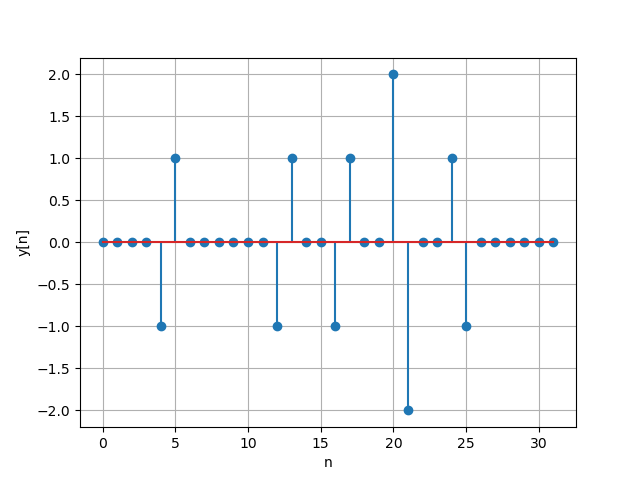
\includegraphics[width=\columnwidth]{./figs/fig.png}
%    \caption{caption}
%    \label{fig: q.no.1}
%\end{figure}

%\end{document}

\pagebreak
\item Consider an ideal full-bridge single-phase DC-AC inverter with a DC bus voltage magnitude of $1000 V$. The inverter output voltage $v(t)$ shown below is obtained when diagonal switches of the inverter are switched with $50\%$ duty cycle. The inverter feeds a load with a sinusoidal current given by $i(t) = 10 \sin(\omega t - \frac{\pi}{3}) \, \mathrm{A}$, where $\omega=\frac{2\pi}{T}$. The active power, in watts, delivered to the load is \underline{\quad}.[Gate2022-EE-58]  \\     
\begin{figure}[htb]
  \centering
  \begin{tikzpicture}
  \begin{axis}[
    xlabel={$t$},
    ylabel={$v(t)$},
    axis lines=middle,
    ymin=-1.5, ymax=1.5,
    xtick={0,0.5,1.0,1.5},
    xticklabels={0, $0.5 T$, $1.0 T$, $1.5 T$},
    ytick={0},
    grid=none,
    enlargelimits=0.2,
    xticklabel style={xshift=-0.4cm},
    height=6cm,
    ]
    \addplot[const plot, thick, blue] coordinates {(0,1) (0.5,1) (0.5,-1) (1,-1) (1,1) (1.5,1)};
  \end{axis}
\end{tikzpicture}




\end{figure}
\solution
\iffalse
\documentclass[journal,12pt,onecolumn]{IEEEtran}
\usepackage{cite}
\usepackage{amsmath,amssymb,amsfonts,amsthm}
\usepackage{algorithmic}
\usepackage{graphicx}
\usepackage{textcomp}
\usepackage{xcolor}
\usepackage{txfonts}
\usepackage{listings}
\usepackage{enumitem}
\usepackage{mathtools}
\usepackage{gensymb}
\usepackage{comment}
\usepackage[breaklinks=true]{hyperref}
\usepackage{tkz-euclide} 
\usepackage{listings}
\def\inputGnumericTable{}                                 
\usepackage[latin1]{inputenc}                                
\usepackage{color}                                            
\usepackage{array}                                            
\usepackage{longtable}                                       
\usepackage{calc}                                             
\usepackage{multirow}                                         
\usepackage{hhline}                                           
\usepackage{ifthen}                                           
\usepackage{lscape}
\usepackage{caption}
\usepackage{subfigure}
\usepackage{gvv}
\usepackage{pgfplots}
\usepackage{circuitikz}
\usepackage{graphicx}

% Define \phase command
\newcommand{\phase}[1]{\text{arg}\left(#1\right)}

\newtheorem{theorem}{Theorem}[section]
\newtheorem{problem}{Problem}
\newtheorem{proposition}{Proposition}[section]
\newtheorem{lemma}{Lemma}[section]
\newtheorem{corollary}[theorem]{Corollary}
\newtheorem{example}{Example}[section]
\newtheorem{definition}[problem]{Definition}
\newcommand{\BEQA}{\begin{eqnarray}}
\newcommand{\EEQA}{\end{eqnarray}}
\newcommand{\system}[1]{\stackrel{#1}{\rightarrow}}
\newcommand{\define}{\stackrel{\triangle}{=}}
\theoremstyle{remark}
\newtheorem{rem}{Remark}

\begin{document}

\bibliographystyle{IEEEtran}
\vspace{3cm}

\title{Gate-2022-EE-58}
\author{EE22BTECH11008 - Annapureddy Siva Meenakshi$^{*}$}
\maketitle
\bigskip

\renewcommand{\thefigure}{\theenumi}
\renewcommand{\thetable}{\theenumi}
Q: Consider an ideal full-bridge single-phase DC-AC inverter with a DC bus voltage magnitude of $1000 V$. The inverter output voltage $v(t)$ shown below is obtained when diagonal switches of the inverter are switched with $50\%$ duty cycle. The inverter feeds a load with a sinusoidal current given by $i(t) = 10 \sin(\omega t - \frac{\pi}{3}) \, \mathrm{A}$, where $\omega=\frac{2\pi}{T}$. The active power, in watts, delivered to the load is \underline{\quad}.[Gate2022-EE-58]  \\     
\begin{figure}[htb]
  \centering
  \begin{tikzpicture}
  \begin{axis}[
    xlabel={$t$},
    ylabel={$v(t)$},
    axis lines=middle,
    ymin=-1.5, ymax=1.5,
    xtick={0,0.5,1.0,1.5},
    xticklabels={0, $0.5 T$, $1.0 T$, $1.5 T$},
    ytick={0},
    grid=none,
    enlargelimits=0.2,
    xticklabel style={xshift=-0.4cm},
    height=6cm,
    ]
    \addplot[const plot, thick, blue] coordinates {(0,1) (0.5,1) (0.5,-1) (1,-1) (1,1) (1.5,1)};
  \end{axis}
\end{tikzpicture}




  \label{fig:EE_58_f1}
\end{figure}
   
\fi
\solution

\begin{table}[!ht]
    \centering
        \begin{tabular}{|c|c|c|} 
    \hline
    \textbf{Variable} & \textbf{Description} & \textbf{Value} \\
    \hline
    $V_\text{s}$ & input DC voltage & $1000V$ \\
    \hline
    $i(t)$ & output current & $\sin(\omega t-\frac{\pi}{3})$ \\
    \hline
    $v(t)$ & Output voltage & given \\
    \hline 
    $\omega$& Frequency &  $\frac{2\pi}{T}$     \\
    \hline
       $v_{0}^{\text{rms}}$&  RMS output voltage at the fundamental frequency& none\\
    \hline
    $i_{\text{rms}}$&  RMS output current at the fundamental frequency& none\\
    \hline
     $v_{0}(t)$&  output voltage at the fundamental frequency& none\\
    \hline
    $\phi$ & phase difference between $v_{0}(t)$ and $i(t)$&none\\
    \hline
    $i_{0}$& amplitude of output current & $1$\\
    \hline
    $P$&        active power delivered&none\\
    \hline
\end{tabular}

    \caption{Input parameters}
    \label{tab:EE_58_t1}
\end{table}

\begin{figure}[htb]
  \centering
  \begin{tikzpicture}

% Draw rectangle for inverter
\draw (0,0) rectangle (2,2);
\node at (1,1) {DC-AC};

% Draw input lines with battery
\draw (-1,1.5) -- (0,1.5) node[midway, left] {};
\draw (-1,0.5) -- (0,0.5) node[midway, left] {};

% Draw output lines
\draw (2,1.5) -- (3,1.5) node[right] {};
\draw (2,0.5) -- (3,0.5) node[right] {};

% Draw load resistor symbol with rotated text
\draw (2.9,0.7) rectangle (3.1,1.3) node[midway, rotate=90] {\rotatebox{-180}{\tiny Load}};

\draw (3,1.3) -- (3,1.5) node[right] {};
\draw (3,0.5) -- (3,0.7) node[right] {};

% Draw battery symbol without arrow and label
\draw (-1,1.5) to [battery1] (-1,0.5);
\node at (-2.1,1) {\tiny $V_\text{s}=1000V DC$};

% Draw current arrow
\draw[->] (3,1.5) -- (3,1.3) node[midway, above] {};

% Add labels for the current arrow
\node at (4.1,1.4) {\tiny $i(t)=\sin(\omega t-\frac{\pi}{3})$};
\node at (2.2,1.4) {\tiny $+$};
\node at (2.2,1) {\tiny $V_0$};
\node at (2.2,0.6) {\tiny $-$};
\end{tikzpicture}


   \captionsetup{justification=centering, singlelinecheck=off}
  \caption{circuit diagram of the system}
  \label{fig:EE_58_f2}
\end{figure}

The Fourier series expansion of the given voltage $v(t)$ is,
\begin{align}
  v(t) &= \sum_{n=1,3,5,\ldots}^{\infty} \frac{4V_{\text{dc}}}{n\pi} \sin(n\omega t)\\
    v_{0}(t)&=  \frac{4V_{\text{dc}}}{\pi} \sin(\omega t)\\
    \therefore \quad \phi &= \frac{\pi}{3}\\
    v_{0}^{\text{rms}}&=  \frac{4V_{\text{dc}}}{\pi \sqrt{2}}\\
    &=\frac{4000}{\pi \sqrt{2}}\\
    i_{\text{rms}}&=\frac{i_{0}}{\sqrt{2}}=\frac{1}{\sqrt{2}}
\end{align}
  Active power delivered to load in Watts is given by,
  \begin{align}
    P &= v_{0}^{\text{rms}} \times i_{\text{rms}} \times \cos{\phi}\\
    &= \frac{4000}{\pi \sqrt{2}} \times \frac{1}{\sqrt{2}} \times \cos{\frac{\pi}{3}}\\
    &\approx 3183 
\end{align}

\begin{figure}[htb]
  \centering
  \begin{tikzpicture}
  \begin{axis}[
    xlabel={$t$},
    ylabel={$v(t)$},
    axis lines=middle,
    ymin=-1.5, ymax=1.5,
    xtick={0,0.5,1.0,1.5},
    xticklabels={0, $0.5 T$, $1.0 T$, $1.5 T$},
    ytick={0},
    grid=none,
    enlargelimits=0.2,
    xticklabel style={xshift=-0.4cm},
    height=6cm,
    ]
    \addplot[const plot, thick, blue] coordinates {(0,1) (0.5,1) (0.5,-1) (1,-1) (1,1) (1.5,1)};
  \end{axis}
\end{tikzpicture}




   \captionsetup{justification=centering, singlelinecheck=off}
  \caption{output voltage and current of the system}
  \label{fig:EE_58_f3}
\end{figure}

%\end{document}


\pagebreak
\item The value of Integral \\
  \begin{align*}
        \oint \brak{\frac{6z}{2z^4-3z^3+7z^2-3z+5}}dz
 \end{align*}
 evaluated over a counter-clockwise circular contour in the complex plane enclosing only the pole $z=\jmath $, where $\jmath$ is the imaginary unit,is
 \begin{enumerate}
     \item $(-1+\jmath)\pi$
     \item $(1+\jmath)\pi$
     \item $2(1-\jmath)\pi$
     \item $(2+\jmath)\pi$
 \end{enumerate}
 \hfill{(GATE 2022 ME)}\\
 \solution\\
 \iffalse
\let\negmedspace\undefined
\let\negthickspace\undefined
\documentclass[journal,12pt,onecolumn]{IEEEtran}
\usepackage{cite}
\usepackage{amsmath,amssymb,amsfonts,amsthm}
\usepackage{algorithmic}
\usepackage{graphicx}
\usepackage{textcomp}
\usepackage{xcolor}
\usepackage{txfonts}
\usepackage{listings}
\usepackage{enumitem}
\usepackage{mathtools}
\usepackage{gensymb}
\usepackage{comment}
\usepackage[breaklinks=true]{hyperref}
\usepackage{tkz-euclide} 
\usepackage{listings}
\usepackage{gvv}                                        
\def\inputGnumericTable{}                                 
\usepackage[latin1]{inputenc}                                
\usepackage{color}                                            
\usepackage{array}                                            
\usepackage{longtable}                                       
\usepackage{calc}                                             
\usepackage{multirow}                                         
\usepackage{hhline}                                           
\usepackage{ifthen}                                           
\usepackage{lscape}

\newtheorem{theorem}{Theorem}[section]
\newtheorem{problem}{Problem}
\newtheorem{proposition}{Proposition}[section]
\newtheorem{lemma}{Lemma}[section]
\newtheorem{corollary}[theorem]{Corollary}
\newtheorem{example}{Example}[section]
\newtheorem{definition}[problem]{Definition}
\newcommand{\BEQA}{\begin{eqnarray}}
 \newcommand{\EEQA}{\end{eqnarray}}
\newcommand{\define}{\stackrel{\triangle}{=}}
\theoremstyle{remark}
\newtheorem{rem}{Remark}
\begin{document}
 \bibliographystyle{IEEEtran}
 \vspace{3cm}
 \title{\textbf{ME 36}}
 \author{EE23BTECH11048-Ponugumati Venkata Chanakya$^{*}$% <-this % stops a space
 }
 \maketitle

 \bigskip
 \renewcommand{\thefigure}{\theenumi}
 \renewcommand{\thetable}{\theenumi}
 \textbf{QUESTION:}
 The value of Integral \\
  \begin{align*}
        \oint \brak{\frac{6z}{2z^4-3z^3+7z^2-3z+5}}dz
 \end{align*}
 evaluated over a counter-clockwise circular contour in the complex plane enclosing only the pole $z=\jmath $, where $\jmath$ is the imaginary unit,is
 \begin{enumerate}
     \item $(-1+\jmath)\pi$
     \item $(1+\jmath)\pi$
     \item $2(1-\jmath)\pi$
     \item $(2+\jmath)\pi$
 \end{enumerate}
 \hfill{(GATE 2022 ME)}\\
 \solution\\
\fi
 Given $z=\jmath$ is only enclosing pole 
 \begin{align}
 \oint \brak{\frac{6z}{2z^4-3z^3+7z^2-3z+5}}dz
 &=\oint \brak{\frac{\frac{6z}{2z^3+(2\jmath-3)z^2+(5-3\jmath)z+5\jmath}}{z-\jmath}}dz\\
 &=2\pi \jmath\brak{\frac{6z}{2z^3+(2\jmath-3)z^2+(5-3\jmath)z+5\jmath}} \text{ At }z=\jmath
    \text{ (Cauchy's integral formula)}\\
    &=2\pi \jmath\brak{\frac{6\jmath}{2\jmath^3+(2\jmath-3)\jmath^2+(5-3\jmath)\jmath+5\jmath}}\\
    &=2\pi \jmath\brak{\frac{\jmath}{\jmath+1}}\\
    &=-2\pi \frac{\jmath-1}{\jmath^2-1}\\
    &=(-1+\jmath)\pi
    \end{align}
 %\end{document}


 \pagebreak
\end{enumerate}
